%%***************************************************
\documentclass[a4paper,12pt]{article}

%% PACKAGES
\usepackage{amssymb}% to have some extra types of fonts
\usepackage{amsmath}
\usepackage{enumitem}
\usepackage{graphicx}
%% - writing in Spanish
\usepackage[latin1]{inputenc}% To type Spanish accents
\usepackage[spanish]{babel}% to have Spanish captions
%% - doc. formatting
\usepackage[a4paper,left=3.1cm,right=3.1cm,bottom=2.5cm,top=2.5cm]{geometry}
\usepackage{fancyhdr}
\pagestyle{fancy}
\fancyhf{}
\newcommand{\notperpg}{\mathrel{\not\!\perp_g}}

\fancyhead[L]{Universidad de Cantabria}    % L = Left
\fancyhead[C]{Grado en Matemáticas}       % C = Center
\fancyhead[R]{Grado en Ing. Informática}      % R = Right
\fancyfoot[R]{\thepage}

\title{Representación del conocimiento \\ Práctica 1}
\author{Víctor Castañeda Balmori, Mario Cuesta Rivavelarde, \\
Carlos García Arenal, Laro Ayesa Sánchez y Alexandru Solovei Popa}
\date{03/10/2025}

\begin{document}

\maketitle
\thispagestyle{fancy}
El objetivo de la práctica es programar el algoritmo que determina si dos nodos de un grafo son separables dado otro conjunto de nodos. Es decir, el algoritmo que determina si $X \perp _g Y \mid Z$. En este documento analizamos la complejidad del código implementado en la carpeta comprimida \textit{practica1.zip}. \\ \\
Para el desarrollo de la práctica hemos dividido el trabajo en el grupo en los 3 pasos del algoritmo. El análisis de la complejidad lo hemos hecho, por tanto, primero por separado cada función (o cada paso con sus funciones) y después en conjunto.

\section{Complejidad del paso 1}

El paso 1 consiste en identificar aquellos nodos que sean nodos hoja, y eliminarlos. Por lo tanto, se recorren todos los nodos (\textbf{n}) y se mantiene una lista con aquellos nodos que aún deban explorarse. Al explorar un nodo, si se elimina de la lista, se vuelven a añadir sus predecesores. En caso contrario, no sucede nada. \\ \\
Así, el peor caso será aquel en que los nodos $\in X \cup Y \cup Z$ (que no pueden ser eliminados) no tengan ningún predecesor y el primer nodo que se pueda eliminar sea el último en ser explorado. En este caso, se explorarán todos los nodos ($O(n)$), y después se irán explorando de nuevo para ir eliminándolos ($O(n)$), resultando un grafo que contenga únicamente los nodos $\in X \cup Y \cup Z$. \\ \\
Con esto tenemos una complejidad temporal de \textbf{2n}, siendo \textbf{n} el número de nodos del grafo. Pero, en cada iteración del bucle, se obtienen los predecesores del nodo que se está explorando. El coste de esta acción es $O(p)$, siendo \textbf{p} el número máximo de predecesores de un nodo. Por lo tanto, $p \le m$. En el caso $p = m$, habrá un solo nodo con predecesores, por lo que este nodo tendrá $n - 1$ predecesores, y la complejidad será de $O(2n*m)$, pero rara vez se dará este caso. \\ \\
Así, la complejidad de eliminar los nodos hoja es la siguiente:
$$O(2n*p) = O(2n*p); \; p \le m$$
donde \textbf{n} es el número de nodos del grafo y \textbf{p} es el número máximo de predecesores de un nodo.

\section{Complejidad del paso 2}
El paso 2 del algoritmo consiste en añadir aristas entre los nodos que tienen el mismo hijo y eliminar la direccionalidad de las aristas. Por lo tanto, el algoritmo que hemos desarrollado consiste en recorrer los nodos del grafo, recorriendo los padres de cada nodo, añadiendo aristas entre los padres con hijos en común. Todo esto, pasando el grafo dirigido a no dirigido. \\ \\
En el peor caso (algo imposible en redes bayesianas) todos los nodos estarán unidos a los demás, de forma que tendrá cada nodo (n-1) padres. De esta forma, tendremos un bucle que recorre todos los nodos O(n). Dentro tendremos un bucle que recorre los padres O(n) y otro dentro de este que también depende de n (siendo n el número de nodos del grafo). En realidad, los dos bucles de los padres dependen de n, pero el de dentro empieza en i + 1 quedándonos una secuencia de iteraciones n + (n-1) + (n-2) + (n-3)... que da lugar a una complejidad $O(n^2/2)$. Sigue dependiendo de n pero es más eficiente. Por lo tanto, \textbf{en el peor caso la complejidad del algoritmo en de $O(n^3)$}. \\ \\ 
Sin embargo, en una red bayesiana no podríamos tener a todos los nodos unidos a todos los demás, por lo que podemos poner una cota de padres máximos que tenga cada hijo (p).La complejidad de los bucles interiores anidados sería $O(p^2/2)$. La complejidad del algoritmo, por tanto, sería $O(n * p^2/2)$ siendo n el número de nodos y p el número máximo de padres de cada nodo.
 
\section{Complejidad del paso 3}
En este último paso, queremos ver si  $X \perp _g Y \mid Z$. Para ello, buscamos eliminar los nodos del conjunto $Z$ (junto a sus aristas), con el propósito de ver si $X$ e $Y$ quedan conectados en el grafo. \\ \\
La complejidad de quitar los nodos de $Z$ es lineal $O(n)$ donde $n$ es el numero de nodos de $Z$, ya que, simplemente hay que recorrer el conjunto y eliminar los nodos. El peor caso es que $Z$ contenga todos los nodos del grafo, menos $X$ e $Y$ en el cual la complejidad es O(E) ya que se eliminan todas las aristas. \\ \\
El peor caso en este paso, ocurre cuando tenemos que visitar todos los nodos porque tendríamos que visitar cada nodo y cada arista. El algoritmo es recursivo pero como guardamos en un conjunto los nodos ya visitados, nos aseguramos que pasaremos solamente una vez por cada nodo. Dicho esto, la complejidad temporal sería  $O(V + E)$, siendo $V$ los nodos del grafo, y $E$, las aristas.

\section{Complejidad Total}
El algoritmo de eliminación de variables consta de llamar a cada una de las tres funciones desarrolladas anteriormente, en el orden en que se han descrito.

Por lo tanto, la complejidad temporal será de $O(np+np^2+(n+m))$. Como $np^2 > np$ se cumplirá siempre, y para un grafo no dirigido el numero maximo de aristas es $\binom{n}{2}$,es decir, una arista por cada pareja de nodos, por lo que la peor complejidad sería $O(np^2 + n^2) = O(np^2)$ siendo el peor caso para $p = \binom{n}{2}$ como en el siguiente ejemplo.

Para comprobar la complejidad total, hemos utilizado un grafo dirigido con $n$ nodos, 
en el que cada nodo $X_i$ (para $i > 0$) es hijo de todos los nodos $X_0, X_1, \dots, X_{i-1}$, 
excepto el nodo $X_0$, que no tiene padres. 
De esta manera, se obtiene el mayor número posible de padres por nodo,  o lo que es lo mismo, el mayor número de aristas en el grafo.

\begin{figure}[h!]
    \centering
    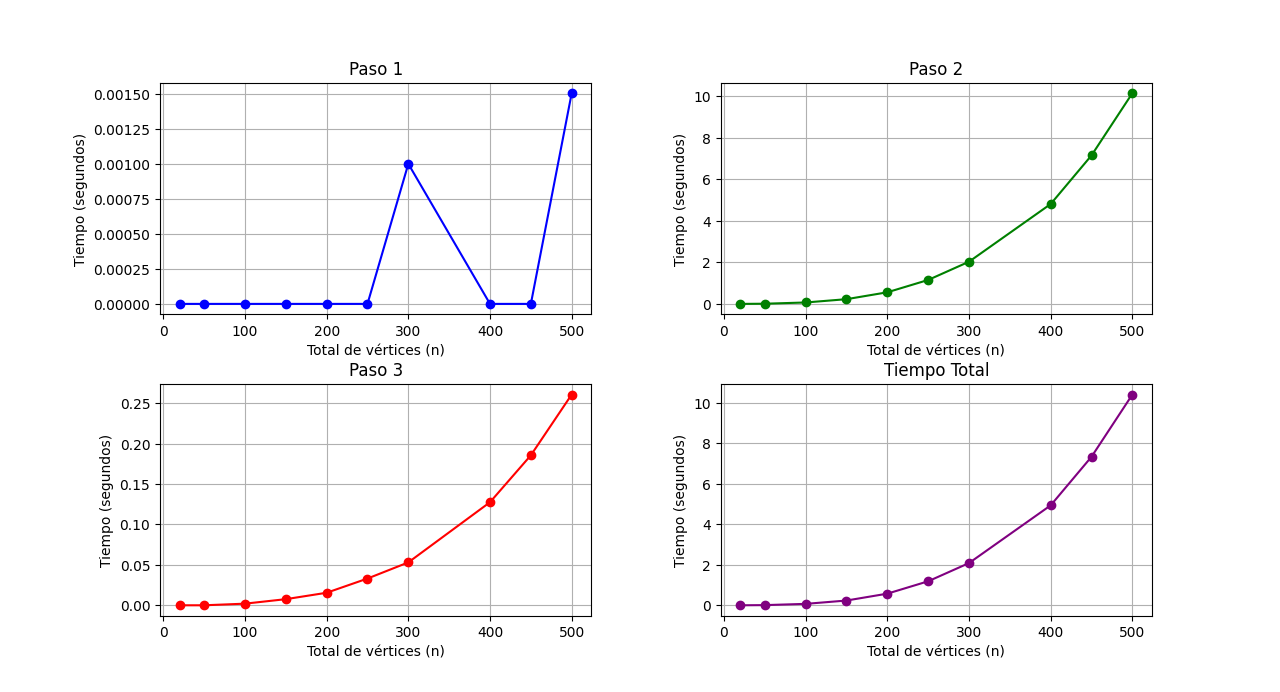
\includegraphics[width=0.8\linewidth]{SinQuitarNodosHoja.png}
    \caption{Peor Caso}
    \label{fig:peorcaso}
\end{figure}

En la Figura \ref{fig:peorcaso} hemos usado como $X$ el primer nodo, como $Y$ un nodo separado de los demás y como $Z$ el nodo $X_i$. De esta manera no hay ningún nodo hoja y el paso 1 tarda poco tiempo. Se dejan todos los nodos para el paso 2 que es el que consume todo el tiempo. El paso 3 tiene que recorrer todas las aristas ya que solo se quita $X_i$ y no va a encontrar camino porque $Y$ esta separado.


\begin{figure}[!h]
    \centering
    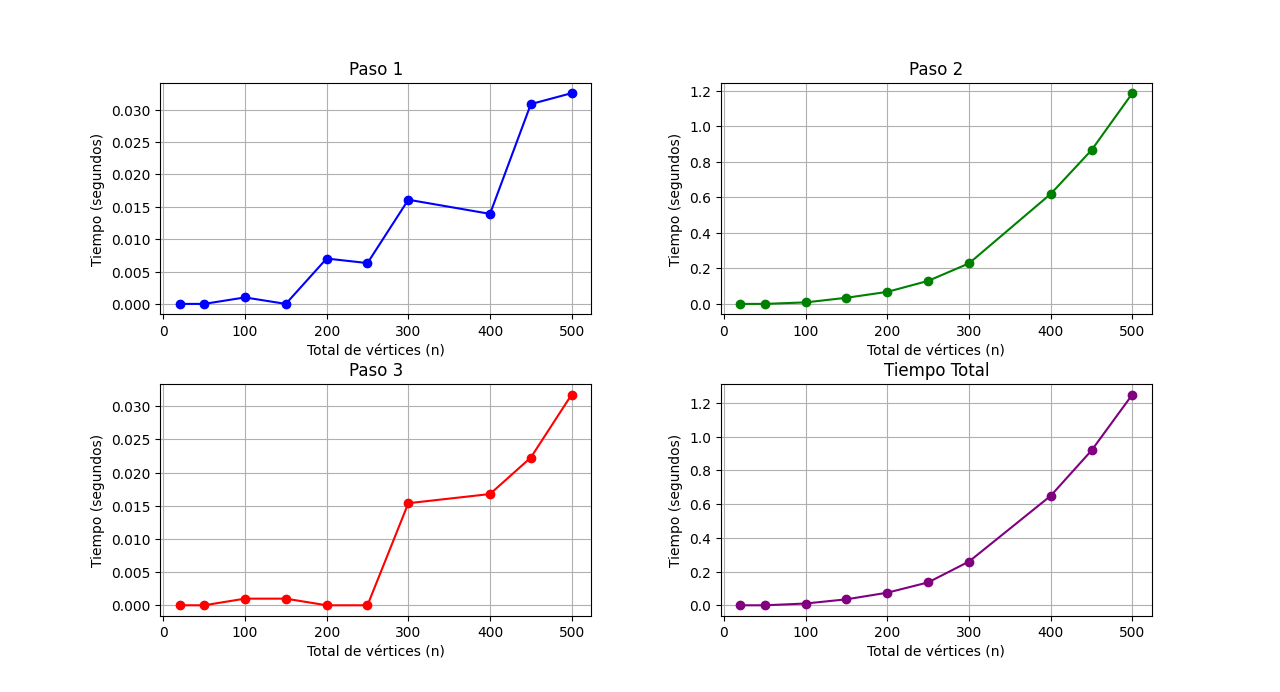
\includegraphics[width=0.8\linewidth]{NodosHojaHastaMitad.png}
    \caption{Con Nodos Hoja}
    \label{fig:nodosHoja}
\end{figure}

En esta Figura \ref{fig:nodosHoja}, $Z = X_{nodos//2}$ por lo que ahora se podrán quitar como nodos hoja la mitad del grafo. Podemos comprobar que el tiempo para 500 nodos se aproxima a el tiempo para 250 nodos de la Figura \ref{fig:peorcaso}. 

\section{Ejemplos del algoritmo de separación}
En el fichero $practica1\_Junto.py$ se han añadido varios ejemplos para probar la eficacia del algoritmo. Cada uno de los ejemplos muestra el estado inicial y la evolución del grafo por cada paso del algoritmo. Los ejemplos se describen a continuación:

\begin{itemize}
    \item Existe un camino entre $X$ e $Y$ sin ningún $Z \in \textbf{Z}$. 
    
    Consecuentemente, $X \notperpg Y \mid \textbf{Z}$.
    
    \item Existe un camino entre $X$ e $Y$ que contiene un $Z \in \textbf{Z}$.

    Consecuentemente, $X \perp _g Y \mid \textbf{Z}$.
    
    \item $X$ e $Y$ se encuentran en componentes conexas distintas.

    Consecuentemente, $X \perp _g Y \mid \textbf{Z}$ para cualquier conjunto $\textbf{Z}$.

    \item Existe más de un camino entre $X$ e $Y$. Todos los caminos contienen un $Z \in \textbf{Z}$.

    Consecuentemente, $X \perp _g Y \mid \textbf{Z}$.

    \item Existe más de un camino entre $X$ e $Y$. Existe al menos
    un camino sin ningún $Z \in \textbf{Z}$.

    Consecuentemente, $X \notperpg Y \mid \textbf{Z}$.
    
\end{itemize}

\end{document}